\subsection{Ton und Tonstufe}
    \textbf{Die Tonstufe} ist ein einzelner Ton einer diatonischen Tonleiter. Als Kernbestand des abendländischen Tonsystems kann man die sieben Tonstufen \textbf{C, D, E, F, G, A und B ansehen, die Stammtöne.} Zwichen den Tonstufen liegt jeweils immer ein Halbtonschritt. Die Tonstufen einer gegebenen Tonleiter werden mit lateinischen Ordinalzahlen benannt.

\begin{table}[H]
    \caption{Tonstufen Steigend}
    \label{tab:TonstufenSteigend}
    \begin{tabularx}{\textwidth}{|>{\hsize=.3\hsize}X|>{\hsize=.3\hsize}X|>{\hsize=.4\hsize}X|}
    \hline
    Halbtönschritte & Ton & lateinische Ordinalzahlen\\ \hline
    0 & \textbf{C} & \textbf{Reine Prime} \\ \hline
    1 & Cis & Kleine Sekunde \\ \hline
    2 & \textbf{D} & \textbf{Große Sekunde} \\ \hline
    3 & Dis & Kleine Terz \\ \hline
    4 & \textbf{E} & \textbf{Große Terz} \\ \hline
    5 & \textbf{F} & \textbf{Quarte} \\ \hline
    6 & Fis & Tritonus \\ \hline
    7 & \textbf{G} & \textbf{Reine Quinte} \\ \hline
    8 & Ais & Kleine Sexte \\ \hline
    9 & \textbf{A} & \textbf{Große Sexte} \\ \hline
    10 & Bb & Kleine Septime \\ \hline
    11 & \textbf{B} & \textbf{Große Septime} \\ \hline
    12 & \textbf{C} & \textbf{Reine Oktave}\\ \hline
    \end{tabularx}
\end{table}

Grundsätzlich betrachten wir die Tonleitern in steigender oder fallender Reihenfolge. Wir erkennen, dass bestimmte Töne zwar verschieden geschrieben werden, jedoch gleich klingen. Ein \textbf{Cis} bspw. klingt wie ein \textbf{Des}. Sie dir dazu mal den Halbtonschritt 1 in der Tabelle \ref{tab:TonstufenSteigend} an und in der Tabelle \ref{tab:TonstufenFallend} den Halbtonschritt 11. Hauptsächlich hat das etwas mit dem Vorzeichen (Versetzungszeichen) zu tun. Das hier erstmal nicht weiter beachtet werden soll.

\begin{table}[H]
    \caption{Tonstufen Fallend}
    \label{tab:TonstufenFallend}
    \begin{tabularx}{\textwidth}{|>{\hsize=.3\hsize}X|>{\hsize=.3\hsize}X|>{\hsize=.4\hsize}X|}
    \hline
    Halbtönschritte & Ton & lateinische Ordinalzahlen\\ \hline
    0 & \textbf{C} & \textbf{Reine Prime} \\ \hline
    1 & B & Kleine Sekunde \\ \hline
    2 & \textbf{Bb} & \textbf{Große Sekunde} \\ \hline
    3 & A & Kleine Terz \\ \hline
    4 & \textbf{As} & \textbf{Große Terz} \\ \hline
    5 & \textbf{G} & \textbf{Quarte} \\ \hline
    6 & Ges & Tritonus \\ \hline
    7 & \textbf{F} & \textbf{Reine Quinte} \\ \hline
    8 & E & Kleine Sexte \\ \hline
    9 & \textbf{Es} & \textbf{Große Sexte} \\ \hline
    10 & D & Kleine Septime \\ \hline
    11 & \textbf{Des} & \textbf{Große Septime} \\ \hline
    12 & \textbf{C} & \textbf{Reine Oktave}\\ \hline
    \end{tabularx}
\end{table}

Wir fassen alle einzelnen Töne noch einmal zusammen. Töne die gleich klingen aber 2 Bezeichnungen haben, werden im Übrigen enharmonische Töne genannt. In der oberen Zeile in Tabelle \ref{tab:ToeneUndHalbtoene} lesen wir die Töne steigend (C, D, E, usw.) und hängen ein -is- an. Wird wie in der unteren Zeile fallend gelesen (C, B, Bb, A, usw.), wird ein -es- angehangen. Aus A wird jedoch As und aus B wird Bb.

\begin{table}[H]
    \caption{Töne und Halbtöne}
    \label{tab:ToeneUndHalbtoene}
    % \begin{tabularx}{\textwidth}{|*{12}{X|}}
    \begin{tabularx}{\textwidth}{|p{1.2cm}|p{1.2cm}|X|X|X|p{1.2cm}|X|X|X|X|X|X|}
    \hline
    \cellcolor{red!25}His/C & \cellcolor{yellow!25}Cis & D & \cellcolor{green!25}Dis & E & \cellcolor{red!25}Eis/F & \cellcolor{gray!25}Fis & G & \cellcolor{blue!25}Gis & A & \cellcolor{orange!25}Ais & B \\ \hline
    C & \cellcolor{red!25}Ces/B & \cellcolor{orange!25}Bb & A & \cellcolor{blue!25}As & G & \cellcolor{gray!25}Ges & F & E & \cellcolor{green!25}Es & D & \cellcolor{yellow!25}Des \\ \hline
    \end{tabularx}
\end{table}

Lass dich von den rot markierten Zellen nicht verwirren. Sie stehen für sich. Lesen wir steigend (also die obere Zeile) und sind beim B angekommen geht es von vorn los und somit ist C auch gleichzeitig ein His. Genauso ist es wenn wir fallend lesen. Hier ist der Ton B und Ces der gleichklingende. Auch zwischen E und F liegt nur ein Halbtonschritt, sodass Eis und F derselbe Ton ist.

\subsection{Tonarten}
Tonarten sind Sequenzen aus natürlichen Tönen mit Vorzeichen. Es gibt zwei Vorzeichen. Das \textbf{Kreuz \# und Das b.} \textbf{Die Anzahl der Töne innerhalb einer Tonleiter die ein -is- bekommen und erhöt werden müssen, entspricht immer der Anzahl der Kreuze \#.} \textbf{Die Anzahl der Töne innerhalb einer Tonleiter die ein -es- bekommen und erniedrigt werden müssen, entspricht immer der Anzahl der b's.} Die Tonart C-Dur besteht komplett aus natürlichen Tönen ohne Vorzeichen: C – D – E – F – G – A – B. Die Tonart G-Dur besteht aus einem Vorzeichen G – A – B – C – D – E – F\#. Im Gegensatz dazu beinhaltet die Tonart \textbf{Cis-Dur} ausschließlich Töne mit Kreuzen: \textbf{C\# – D\# – E\# – F\# – G\# – A\# – B\#.} Erkennen kannst du es immer an den Vorzeichnen die vor dem Notenschlüssel stehen.

\begin{minipage}[b]{0.3\linewidth}
    \begin{figure}[H]
        \centering
        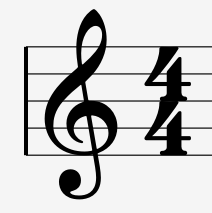
\includegraphics[width=0.4\textwidth]{images/Signiture_2}
        \caption[]{C-Dur}
        \label{fig:CDur}
    \end{figure}
  \end{minipage}
  \begin{minipage}[b]{0.3\linewidth}
    \begin{figure}[H]
        \centering
        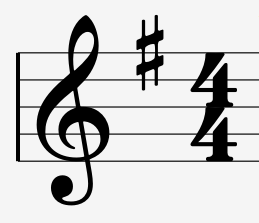
\includegraphics[width=0.45\textwidth]{images/Signiture_3}
        \caption[]{G-Dur}
        \label{fig:GDur}
    \end{figure}
  \end{minipage}
  \begin{minipage}[b]{0.3\linewidth}
    \begin{figure}[H]
        \centering
        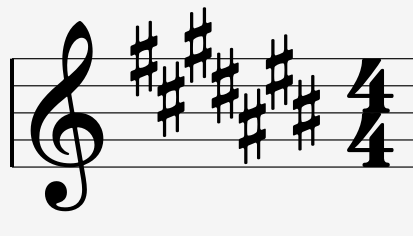
\includegraphics[width=0.65\textwidth]{images/Signiture_1}
        \caption[]{Cis-Dur}
        \label{fig:CisDur}
    \end{figure}
  \end{minipage}

\subsection{Tonleitern}
Eine Tonleiter oder Ton-Skala ist in der Musik eine Reihe von der Tonhöhe nach geordneten Tönen. In den meisten Fällen hat eine Tonleiter den Umfang einer Oktave. Weit verbreitet sind diatonische Tonleitern in Dur und Moll. Tonleitern sind durch Tonabstände definiert. An erster Stelle steht der Grundton (wie zum Beispiel C) nach 8 Tönen (also einer Oktave) wiederholt sich die Reihe. Der 8. Ton ist also wieder ein C. 
\textbf{Die Verbindung des Tongeschlechts, also bspw. Dur oder Moll, mit dem Grundton ergibt die Tonart}. 
C-Dur ist hierfür ein Beispiel. Weitere sind A-Moll, D-Dur usw.

Eine Dur-Tonleiter wird ausgehend vom Grundton gebildet, indem jeweils ein Ganztonschritt weiter 
gesprungen wird. Die \textbf{Stellen von Ton 3 zu 4 und von Ton 7 zu 8. sind Ausnahmen. Hier wird nur ein
Halbtonschritt gesprungen.} Analog wird diese Verfahrensweise auch für alle weiteren Grundtöne angewendet. 
In der Tabelle sind die gebräuchlichsten Dur Tonleitern angegeben. Die Farben markieren den Halbtonschritt. Schau dir genau an welche Töne ein -is- bekommen.

\begin{table}[H]
    \caption{Gebräuchlichste Dur-Tonleitern}
    \label{tab:TonstufenDur}
    \begin{tabularx}{\textwidth}{|*{8}{>{\hsize=.1\hsize}X|}}
    \hline
    1. Ton & 2. Ton & 3. Ton & 4. Ton & 5. Ton & 6. Ton & 7. Ton & 8. Ton \\ \hline  
    C & D & \cellcolor{gray!25}E & \cellcolor{gray!25}F & G & A & \cellcolor{gray!25}B & \cellcolor{gray!25}C \\ \hline  
    Cis & Dis & \cellcolor{gray!25}Eis & \cellcolor{gray!25}Fis & Gis & Ais & \cellcolor{gray!25}Bis & \cellcolor{gray!25}Cis \\ \hline  
    D & E & \cellcolor{gray!25}Fis & \cellcolor{gray!25}G & A & B & \cellcolor{gray!25}Cis & \cellcolor{gray!25}D \\ \hline
    Des & Es & \cellcolor{gray!25}F & \cellcolor{gray!25}Ges & As & Bb & \cellcolor{gray!25}C & \cellcolor{gray!25}Des \\ \hline  
    Es & F & \cellcolor{gray!25}G & \cellcolor{gray!25}As & Bb & C & \cellcolor{gray!25}D & \cellcolor{gray!25}Es \\ \hline  
    F & G & \cellcolor{gray!25}A & \cellcolor{gray!25}Bb & C & D & \cellcolor{gray!25}E & \cellcolor{gray!25}F \\ \hline  
    Fis & Gis & \cellcolor{gray!25}Ais & \cellcolor{gray!25}B & Cis & Dis & \cellcolor{gray!25}Eis & \cellcolor{gray!25}Fis \\ \hline  
    G & A & \cellcolor{gray!25}B & \cellcolor{gray!25}C & D & E & \cellcolor{gray!25}Fis & \cellcolor{gray!25}G \\ \hline  
    A & B & \cellcolor{gray!25}Cis & \cellcolor{gray!25}D & E & Fis & \cellcolor{gray!25}Gis & \cellcolor{gray!25}A \\ \hline  
    B & C & \cellcolor{gray!25}D & \cellcolor{gray!25}Es & F & G & \cellcolor{gray!25}A & \cellcolor{gray!25}Bb \\ \hline  
    H & Cis & \cellcolor{gray!25}Dis & \cellcolor{gray!25}E & Fis & Gis & \cellcolor{gray!25}Ais & \cellcolor{gray!25}Bb \\ \hline  
    \end{tabularx}
\end{table}

Eine Moll-Tonleiter wird  gebildet, ausgehend vom Grundton, indem jeweils ein Ganztonschritt weiter 
gesprungen wird. Die \textbf{Stellen von Ton 2 zu 3 und vom Ton 5 zu 6.} sind Ausnahmen. Hier wird nur ein
Halbtonschritt gesprungen. Analog wird diese Verfahrensweise auch für alle weiteren Grundtöne angewendet. 
In der Tabelle \ref{tab:TonstufenMoll} sind die gebräuchlichsten Moll Tonleitern angegeben. Die Farben markieren den Halbtonschritt.


\begin{table}[H]
    \caption{Gebräuchlichste Moll-Tonleitern}
    \label{tab:TonstufenMoll}
    \begin{tabularx}{\textwidth}{|*{8}{>{\hsize=.1\hsize}X|}}
    \hline
    1. Ton & 2. Ton & 3. Ton & 4. Ton & 5. Ton & 6. Ton & 7. Ton & 8. Ton \\ \hline
    C & \cellcolor{gray!25}D & \cellcolor{gray!25}Es & F & \cellcolor{gray!25}G & \cellcolor{gray!25}As & Bb & C \\ \hline
    Cis & \cellcolor{gray!25}Dis & \cellcolor{gray!25}E & Fis & \cellcolor{gray!25}Gis & \cellcolor{gray!25}A & B & Cis \\ \hline
    D & \cellcolor{gray!25}E & \cellcolor{gray!25}F & G & \cellcolor{gray!25}A & \cellcolor{gray!25}Bb & C & D \\ \hline
    Dis & \cellcolor{gray!25}Eis & \cellcolor{gray!25}Fis & Gis & \cellcolor{gray!25}Ais & \cellcolor{gray!25}B & Cis & Dis \\ \hline
    E & \cellcolor{gray!25}Fis & \cellcolor{gray!25}G & A & \cellcolor{gray!25}B & \cellcolor{gray!25}C & D & E \\ \hline
    F & \cellcolor{gray!25}G & \cellcolor{gray!25}As & Bb & \cellcolor{gray!25}C & \cellcolor{gray!25}Des & Es & F \\ \hline
    Fis & \cellcolor{gray!25}Gis & \cellcolor{gray!25}A & B & \cellcolor{gray!25}Cis & \cellcolor{gray!25}D & E & Fis \\ \hline
    G & \cellcolor{gray!25}A & \cellcolor{gray!25}Bb & C & \cellcolor{gray!25}D & \cellcolor{gray!25}Es & F & G \\ \hline
    Gis & \cellcolor{gray!25}Ais & \cellcolor{gray!25}B & Cis & \cellcolor{gray!25}Dis & \cellcolor{gray!25}E & Fis & Gis \\ \hline
    As & \cellcolor{gray!25}Bb & \cellcolor{gray!25}Ces & Des & \cellcolor{gray!25}Es & \cellcolor{gray!25}Fes & Ges & As \\ \hline
    A & \cellcolor{gray!25}B & \cellcolor{gray!25}C & D & \cellcolor{gray!25}E & \cellcolor{gray!25}F & G & A \\ \hline
    B & \cellcolor{gray!25}C & \cellcolor{gray!25}Des & Es & \cellcolor{gray!25}F & \cellcolor{gray!25}Ges & As & Bb \\ \hline
    H & \cellcolor{gray!25}Cis & \cellcolor{gray!25}D & E & \cellcolor{gray!25}Fis & \cellcolor{gray!25}G & A & B \\ \hline
    \end{tabularx}
\end{table}